\subsection{Opacity measurement consistency tests}

%{\bf copy from the 'Instru' paper}

We observe {\bf FM: where ?} that the skydip-fitted $\tau$ values are, as expected,
common between different detectors of the same array. By comparing
the results of different skydips, we have verified experimentally
that the coefficients $C_0$, $C_1$ are stable, within the fit
errors, on very long time scales within a cooldown cycle. The
coefficients can thus be applied to the whole observing campaign
in order to recover the opacity of each scan.


\noindent {\bf FM : a figure would help to convince the reader that it is stable on lng time
scale, which is a key point.}\\


\begin{figure}[ht]
\begin{center}
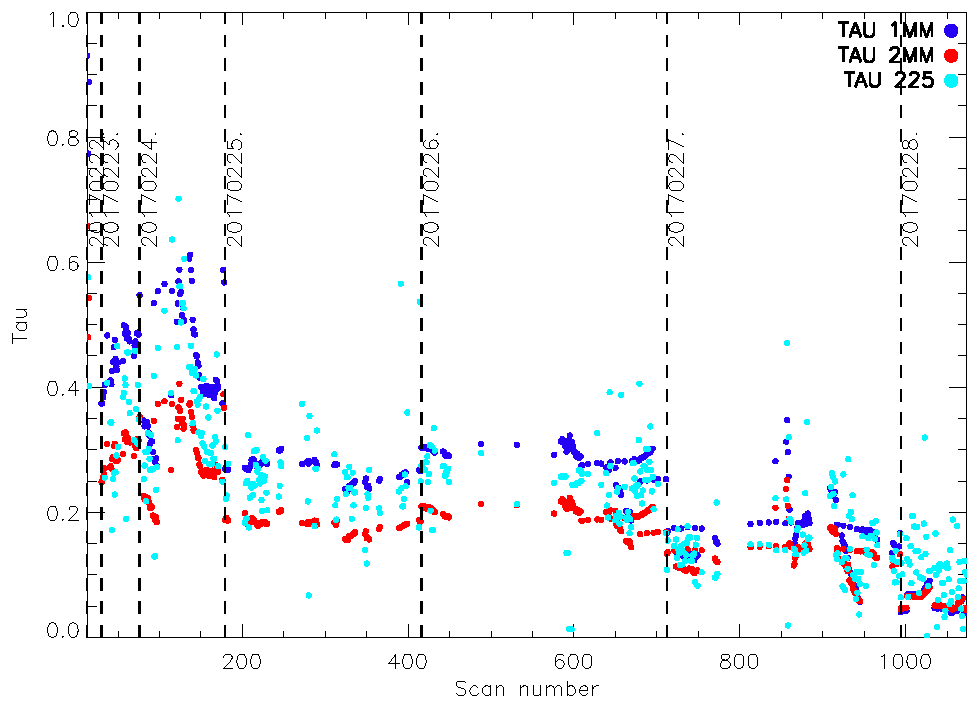
\includegraphics[scale=0.8]{../../Paper_NIKA2_Technical/opacity_evol_run22.pdf}
\caption{Atmospheric opacity as measured from the IRAM 225\,GHz taumeter (cyan), and from the NIKA2 data at 150 (red) and 260\,GHz (blue) during 
  N2R9 commissioning campaign (Feb. 2017). We stress the fact that the IRAM 225\,GHz taumeter data is not used for the atmospheric correction and is plotted here just for comparison.
  \label{fig:taumeas_paper}}
\end{center}
\end{figure}



\begin{figure}[ht]
\begin{center}
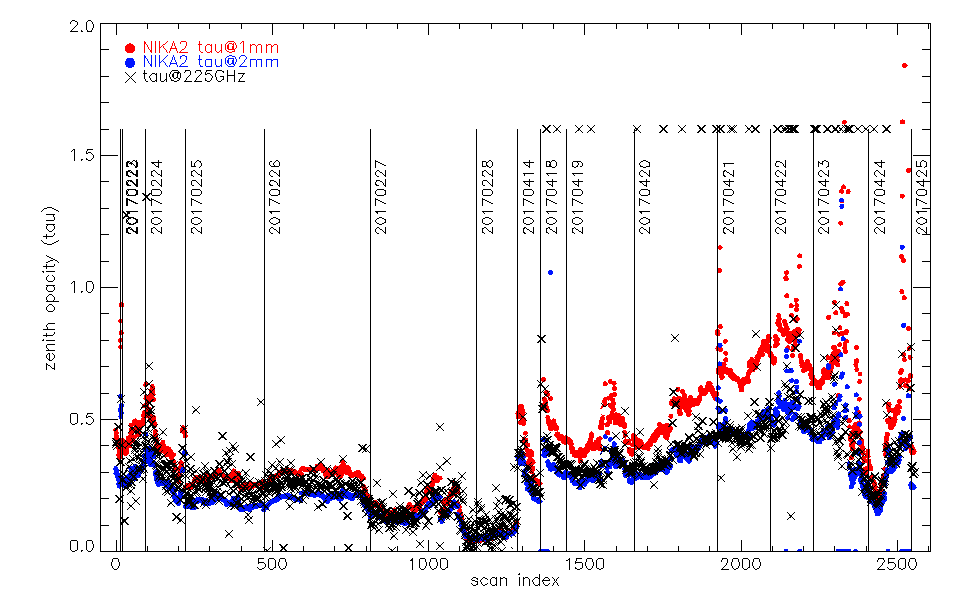
\includegraphics[width=\linewidth]{Figures/opacity_vs_index_N2R9_N2R10.png}
\caption{Atmospheric opacity as measured from the IRAM 225\,GHz
  taumeter (black crosses), and from the NIKA2 data at 150 (red) and 260\,GHz (blue) during 
  N2R9 and N2R10 commissioning campaigns.  We stress the fact that the IRAM 225\,GHz taumeter data is not used for the atmospheric correction and is plotted here just for comparison.
  \label{fig:taumeas}}
\end{center}
\end{figure}


In Fig.~\ref{fig:taumeas} {\bf(and Fig.~\ref{fig:taumeas_paper} of
  \ref{NIKA2-Tech}) } we present the evolution of the NIKA2 in-band
opacities for all the 'OTF' scans (about 1300 scans per runs) of the
N2R9 run held in February and the N2R10 run in April 2017. These are
compared to the IRAM tau-meter values. We observe an agreement on the global trend between the IRAM tau-meter opacity
(225 GHz) and the NIKA2 values. These latter show, however,
a smaller dispersion {\bf FM : how small ?}.


{\bf In  \ref{NIKA2-Tech}, one can read:}  
``We find an average ratio between the
150 GHz and the 260 GHz NIKA2 values of about
0.6, consistent with model expectations. We notice however that
the 150 GHz-to-260 GHz opacity ratio varies significantly for
opacities (at 150 GHz) below 0.2. This effect is likely to be
linked to an $O_2$ atmospheric line which becomes saturated. This
point is, however, still under investigation.''


\noindent {\bf FM : a figure of the ratio of taus would be useful. It should be compared with  
Fig. \ref{thopacities}, which should appear in this section ...}



\begin{figure}[ht]
\begin{center}
  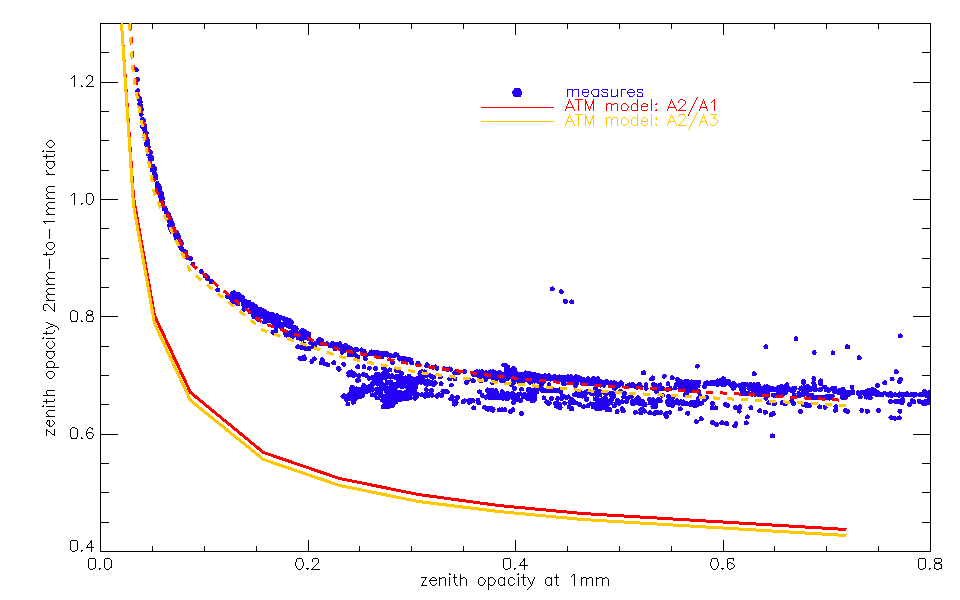
\includegraphics[width=0.65\textwidth]{Figures/opacity_tau1_tau2_ratio_N2R9_N2R10.png}
  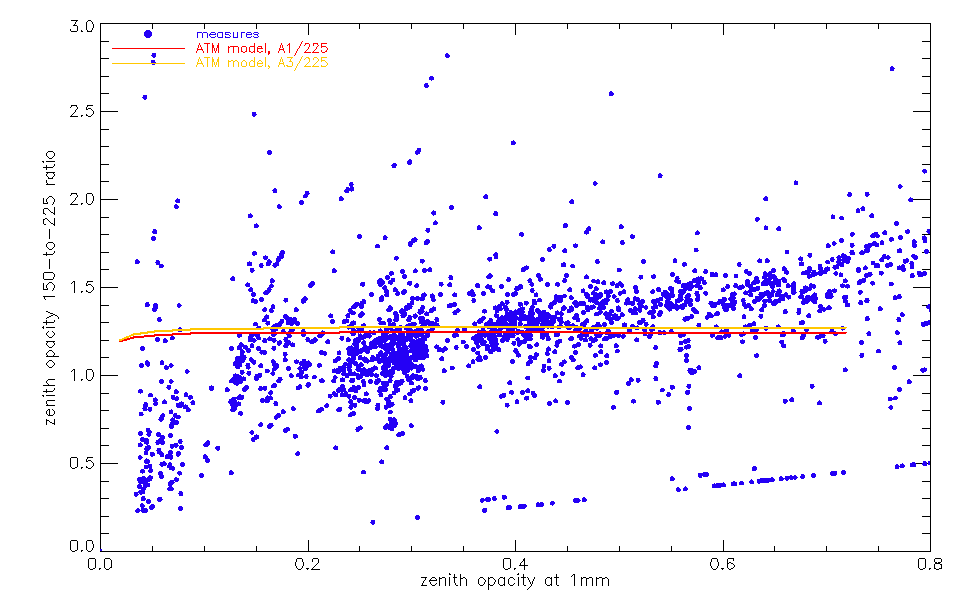
\includegraphics[width=0.65\textwidth]{Figures/opacity_tau1_tau225_ratio_N2R9_N2R10.png}
  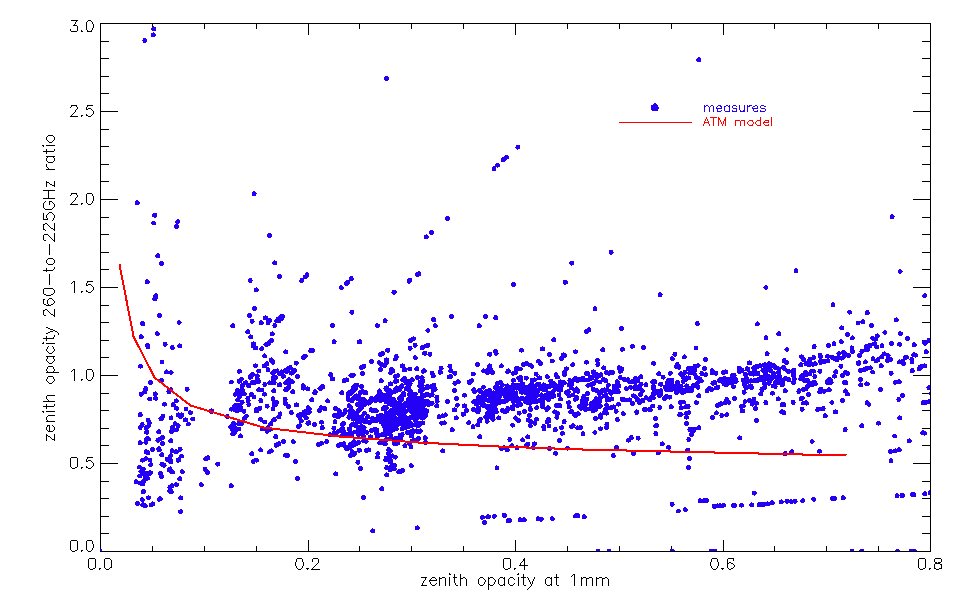
\includegraphics[width=0.65\textwidth]{Figures/opacity_tau2_tau225_ratio_N2R9_N2R10.png}
\caption{Ratios between the 150 GHz and the 260 GHz NIKA2 zenith opacity
estimates and between the NIKA2 $\tau$ and the IRAM taumeter
values. The expectation values derived for NIKA2 bands
using the ATM model described in \ref{Pardo2002} are shown for
comparison (red and orange curves).}
  \label{fig:opacity_ratios}
\end{center}
\end{figure}

\begin{figure}[ht]
\begin{center}
  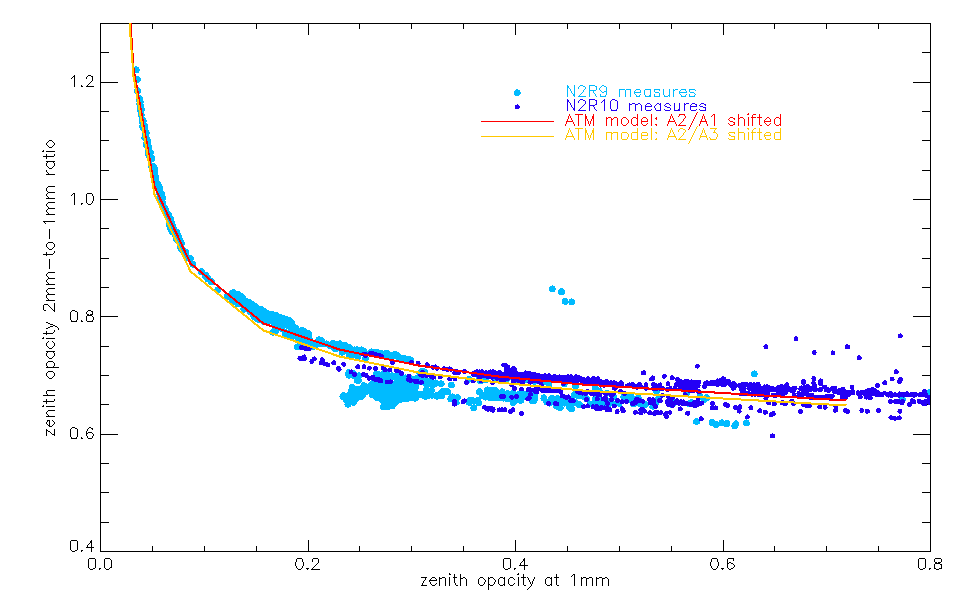
\includegraphics[width=0.8\textwidth]{Figures/opacity_tau1_tau2_byrun_ratio_N2R9_N2R10.png}
  \caption{Ratio between the 150 GHz and the 260 GHz NIKA2 zenith opacity
estimates. The expectation values derived for NIKA2 bands
using the ATM model described in \ref{Pardo2002} are shown for
comparison (red and orange curves). The observed NIKA2 opacity ratio
has a smooth, consistent behaviour over the overall probed opacity range,
and very few outlier estimates are seen although no scan selection has
been performed (out from discarding the dark tests). Also remarkable
is the consistency between estimates obtained during two campaigns
held two months apart in different weather conditions (good to average
during N2R9 and poor and often hightly unstable conditions during
N2R10). Some sub-structures are seen in the opacity ratio, which are
under investigations. They can have several origins (telescope cabin
temperature variation, variation of the $0_2$ fraction, atmospheric
temperature variation, internal temperature variations, etc).  
  }
  \label{fig:opacity_ratios}
\end{center}
\end{figure}

\begin{figure}[ht]
\begin{center}
  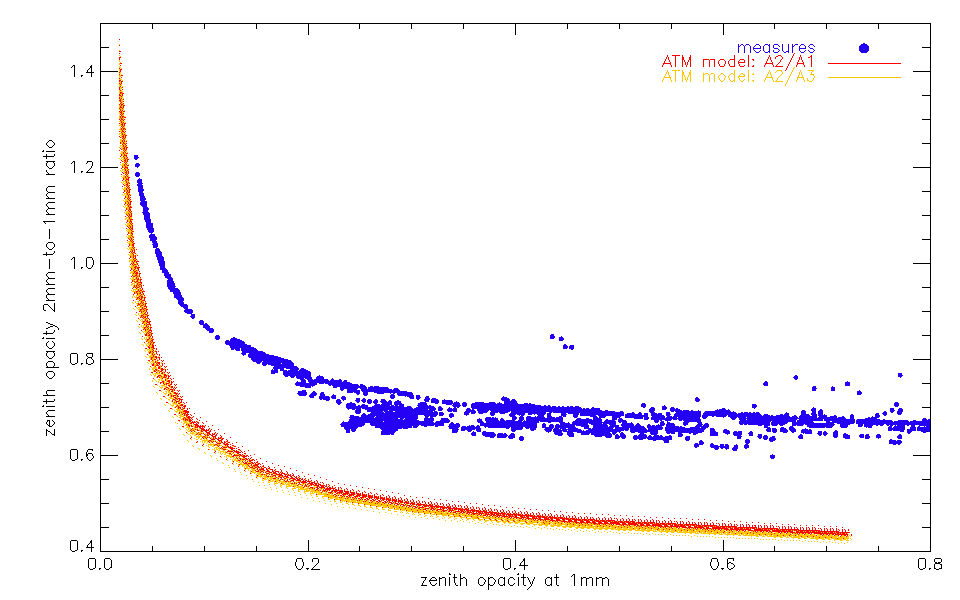
\includegraphics[width=0.8\textwidth]{Figures/opacity_tau1_tau2_ratio_bperror10pc_N2R9_N2R10.png}
  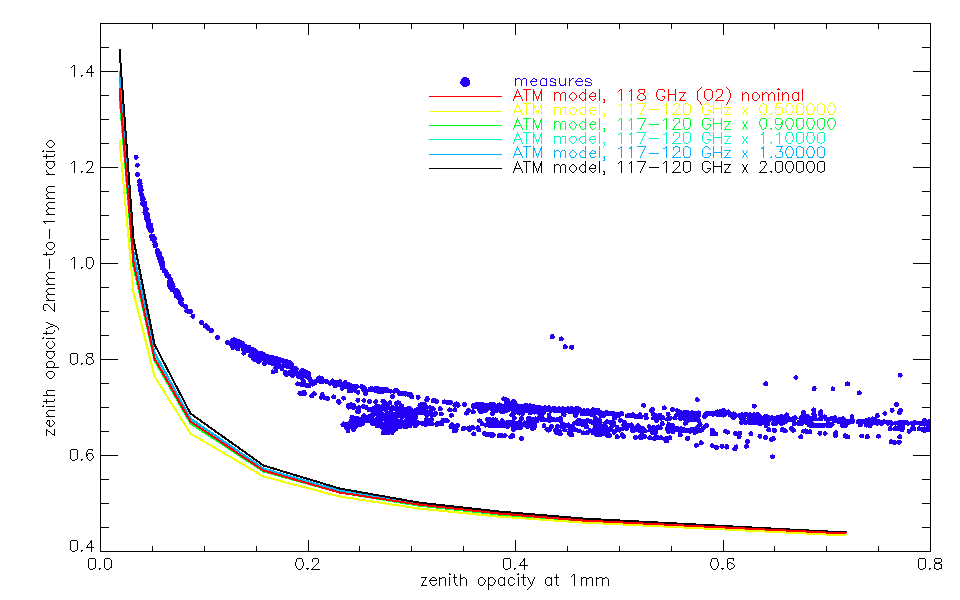
\includegraphics[width=0.8\textwidth]{Figures/opacity_tau1_tau2_ratio_o2fraction_N2R9_N2R10.png}
\caption{Uncertainty of NIKA2 $\tau$ values. Upper panel: The impact
  of the NIKA2 transmission measurement uncertainties is illustrated
  using a very pessimistic relative uncertainty of $10\%$ (instead of
  the more realistic $1\%$ errors). Lower panel: The impact of the
uncertainty on the atmospheric absorption around $118\, \rm{GHz}$, due
to the lack of precise knowledge of the fraction of oxygene in the
atmosphere. The nominal absorption predicted by the ATM model is
modified by a factor from 0.5 to 2 in the $117-120\, \rm{GHz}$
frequency band, where the $0_2$ contributions largely dominates the
water vapor ones. }
  \label{fig:opacity_errors}
\end{center}
\end{figure}

\begin{figure}[ht]
\begin{center}
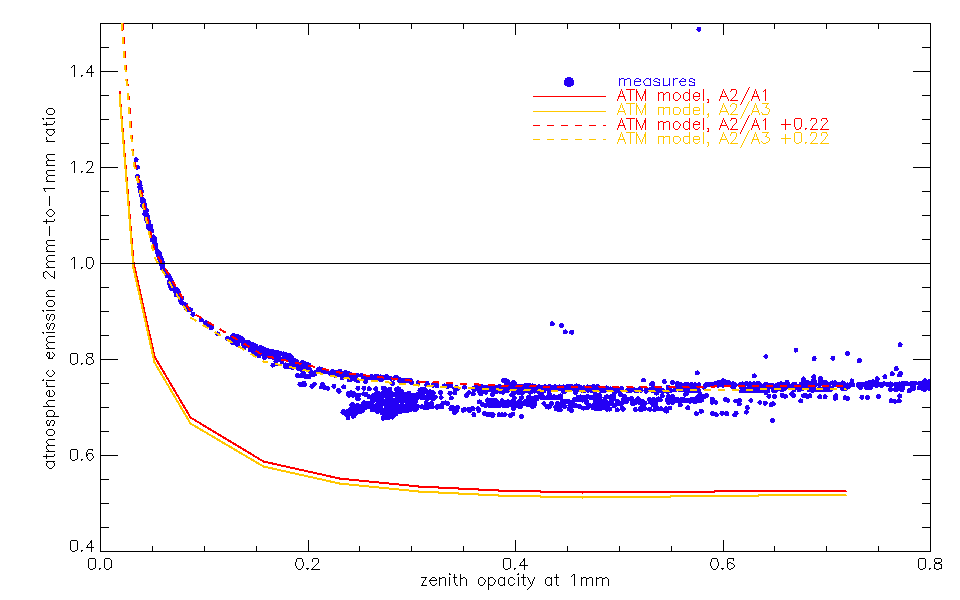
\includegraphics[width=0.9\textwidth]{Figures/opacity_tau1_tau2_emissionratio_N2R9_N2R10.png}
\caption{Ratio of the atmospheric emission in NIKA2 bands defined as
  in Eq.~\ref{eq:opacity_emission_ratio}, compared with the ATM-model
  predicted ratio calculated as in Eq.~\ref{eq:opacity_emission_ratio_model}}
  \label{fig:opacity_emission}
\end{center}
\end{figure}

The ratios between the 150 GHz and the 260 GHz NIKA2 zenith opacity
estimates, quoted $\tau_{2mm}$ and $\tau_{1mm}$ , and
between the NIKA2 $\tau$ and the IRAM taumeter values are presented in
Fig.~\ref{opacity_ratios}, along with the expectation values derived for NIKA2 bands
using the ATM model described in \ref{Pardo2002}. Namely, these
predicted values $\tau^{th}$ are calculated from the ATM-model
atmospheric zenith opacity $\tau^{ATM}$ using:  
\begin{equation}
  \tau^{th}_{A_i} = - \ln{\frac{\int e^{-\tau^{ATM}(\nu)}
      T_{A_i}(\nu) d\nu}{ \int T_{A_i}(\nu) d\nu}},
\end{equation}

where the NIKA2 bandpasses $T_{A_i}$ for arrays $A_i$, $i=1, 2, 3$, are the Martin-Pupplet reference transmissions
corrected by a Rayleigh-Jeans term  $T'_{A_i}(\nu) /
\left( \frac{\nu}{\nu_0}\right)^2$. 

In Fig.~\ref{fig:opacity_emission}, we
show the ratio of the atmospheric emission in NIKA2 bands defined as:
\begin{equation}
  R_{\rm{atm}} = \frac{1-e^{-\tau_{2mm}}}{1-e^{-\tau_{1mm}}}.
    \label{eq:opacity_emission_ratio}
\end{equation}

It is compared with the ATM-model predicted ratio
\begin{equation}
  R_{\rm{atm}}^{th} = \frac{\int (1 - e^{-\tau^{\rm{ATM}}}) T_{A_2}(\nu) d\nu }{\int T_{A_2}(\nu) d\nu} / \frac{\int (1 -
      e^{-\tau^{\rm{ATM}}}) T_{A_{1}}(\nu) d\nu }{\int T_{A_1}(\nu)
        d\nu} .
      \label{eq:opacity_emission_ratio_model}
\end{equation}

In Fig.~\ref{fig:opacity_errors}, we investigate different effects that can impact the precision with
which the zenith opacities are determined: the upper panel shows the
expected dispersion in the NIKA2 $\tau$ values coming from the transmission
measurement uncertainties: to higlight this effect, we consider a very
pessimistic relative uncertainty of $10\%$ (whereas $1\%$ would have
been a more realistic value), and the lower panel shows the impact of the
uncertainty on the fraction of oxygene in the atmosphere, which mainly 
translates in an uncertainty on the atmospheric absorption around
$118\, \rm{GHz}$: the nominal absorption predicted by the ATM model is
modified by a factor from 0.5 to 2 in the $117-120\, \rm{GHz}$
frequency band, where the $0_2$ contributions largely dominates the
water vapor ones. 



